%%%%%%%%%%%%%%%%%%%%%%%%%%%%%%%%%%%%%%%%%
% Thesis 
% LaTeX Template
% Version 1.3 (21/12/12)
%
% This template has been downloaded from:
% http://www.latextemplates.com
%
% Original authors:
% Steven Gunn 
% http://users.ecs.soton.ac.uk/srg/softwaretools/document/templates/
% and
% Sunil Patel
% http://www.sunilpatel.co.uk/thesis-template/
%
% License:
% CC BY-NC-SA 3.0 (http://creativecommons.org/licenses/by-nc-sa/3.0/)
%
% Note:
% Make sure to edit document variables in the Thesis.cls file
%
%%%%%%%%%%%%%%%%%%%%%%%%%%%%%%%%%%%%%%%%%

%----------------------------------------------------------------------------------------
%	PACKAGES AND OTHER DOCUMENT CONFIGURATIONS
%----------------------------------------------------------------------------------------

\documentclass[11pt, a4paper, oneside]{Thesis} % Paper size, default font size and one-sided paper

\graphicspath{{./Pictures/}} % Specifies the directory where pictures are stored

\usepackage[utf8]{inputenc}
\usepackage[square, numbers, comma, sort&compress]{natbib} % Use the natbib reference package - read up on this to edit the reference style; if you want text (e.g. Smith et al., 2012) for the in-text references (instead of numbers), remove 'numbers' 
\hypersetup{urlcolor=blue, colorlinks=true} % Colors hyperlinks in blue - change to black if annoying
\title{\ttitle} % Defines the thesis title - don't touch this

\begin{document}

\frontmatter % Use roman page numbering style (i, ii, iii, iv...) for the pre-content pages

\setstretch{1.3} % Line spacing of 1.3

% Define the page headers using the FancyHdr package and set up for one-sided printing
\fancyhead{} % Clears all page headers and footers
\rhead{\thepage} % Sets the right side header to show the page number
\lhead{} % Clears the left side page header

\pagestyle{fancy} % Finally, use the "fancy" page style to implement the FancyHdr headers

\newcommand{\HRule}{\rule{\linewidth}{0.5mm}} % New command to make the lines in the title page

% PDF meta-data
\hypersetup{pdftitle={\ttitle}}
\hypersetup{pdfsubject=\subjectname}
\hypersetup{pdfauthor=\authornames}
\hypersetup{pdfkeywords=\keywordnames}

%----------------------------------------------------------------------------------------
%	TITLE PAGE
%----------------------------------------------------------------------------------------

\begin{titlepage}
\begin{center}

\textsc{\LARGE \univname}\\[1.5cm] % University name
\textsc{\Large Bachelor Thesis}\\[0.5cm] % Thesis type

\HRule \\[0.4cm] % Horizontal line
{\huge \bfseries \ttitle}\\[0.4cm] % Thesis title
\HRule \\[1.5cm] % Horizontal line
 
\begin{minipage}{0.4\textwidth}
\begin{flushleft} \large
\emph{Author:}\\
\href{http://www.johnsmith.com}{\authornames} % Author name - remove the \href bracket to remove the link
\end{flushleft}
\end{minipage}
\begin{minipage}{0.4\textwidth}
\begin{flushright} \large
\emph{Supervisor:} \\
\href{http://www.jamessmith.com}{\supname} % Supervisor name - remove the \href bracket to remove the link  
\end{flushright}
\end{minipage}\\[3cm]
 
\large \textit{A thesis submitted in fulfilment of the requirements\\ for the degree of \degreename}\\[0.3cm] % University requirement text
\textit{in the}\\[0.4cm]
\groupname\\\deptname\\[2cm] % Research group name and department name
 
{\large \today}\\[4cm] % Date
%\includegraphics{Logo} % University/department logo - uncomment to place it
 
\vfill
\end{center}

\end{titlepage}

%----------------------------------------------------------------------------------------
%	DECLARATION PAGE
%	Your institution may give you a different text to place here
%----------------------------------------------------------------------------------------

\Declaration{

\addtocontents{toc}{\vspace{1em}} % Add a gap in the Contents, for aesthetics

I, \authornames, declare that this thesis titled, '\ttitle' and the work presented in it are my own. I confirm that:

\begin{itemize} 
\item[\tiny{$\blacksquare$}] This work was done wholly or mainly while in candidature for a research degree at this University.
\item[\tiny{$\blacksquare$}] Where any part of this thesis has previously been submitted for a degree or any other qualification at this University or any other institution, this has been clearly stated.
\item[\tiny{$\blacksquare$}] Where I have consulted the published work of others, this is always clearly attributed.
\item[\tiny{$\blacksquare$}] Where I have quoted from the work of others, the source is always given. With the exception of such quotations, this thesis is entirely my own work.
\item[\tiny{$\blacksquare$}] I have acknowledged all main sources of help.
\item[\tiny{$\blacksquare$}] Where the thesis is based on work done by myself jointly with others, I have made clear exactly what was done by others and what I have contributed myself.\\
\end{itemize}
 
Signed:\\
\rule[1em]{25em}{0.5pt} % This prints a line for the signature
 
Date:\\
\rule[1em]{25em}{0.5pt} % This prints a line to write the date
}

\clearpage % Start a new page

%----------------------------------------------------------------------------------------
%	QUOTATION PAGE
%----------------------------------------------------------------------------------------

\pagestyle{empty} % No headers or footers for the following pages

\null\vfill % Add some space to move the quote down the page a bit

\textit{``Thanks to my solid academic training, today I can write hundreds of words on virtually any topic without possessing a shred of information, which is how I got a good job in journalism."}

\begin{flushright}
Dave Barry
\end{flushright}

\vfill\vfill\vfill\vfill\vfill\vfill\null % Add some space at the bottom to position the quote just right

\clearpage % Start a new page

%----------------------------------------------------------------------------------------
%	ABSTRACT PAGE
%----------------------------------------------------------------------------------------

\addtotoc{Abstract} % Add the "Abstract" page entry to the Contents

\abstract{\addtocontents{toc}{\vspace{1em}} % Add a gap in the Contents, for aesthetics

The Thesis Abstract is written here (and usually kept to just this page). The page is kept centered vertically so can expand into the blank space above the title too\ldots
}

\clearpage % Start a new page

%----------------------------------------------------------------------------------------
%	ACKNOWLEDGEMENTS
%----------------------------------------------------------------------------------------

\setstretch{1.3} % Reset the line-spacing to 1.3 for body text (if it has changed)

\acknowledgements{\addtocontents{toc}{\vspace{1em}} % Add a gap in the Contents, for aesthetics

The acknowledgements and the people to thank go here, don't forget to include your project advisor\ldots
}
\clearpage % Start a new page

%----------------------------------------------------------------------------------------
%	LIST OF CONTENTS/FIGURES/TABLES PAGES
%----------------------------------------------------------------------------------------

\pagestyle{fancy} % The page style headers have been "empty" all this time, now use the "fancy" headers as defined before to bring them back

\lhead{\emph{Contents}} % Set the left side page header to "Contents"
\tableofcontents % Write out the Table of Contents

\lhead{\emph{List of Figures}} % Set the left side page header to "List of Figures"
\listoffigures % Write out the List of Figures

\lhead{\emph{List of Tables}} % Set the left side page header to "List of Tables"
\listoftables % Write out the List of Tables

%----------------------------------------------------------------------------------------
%	ABBREVIATIONS
%----------------------------------------------------------------------------------------

\clearpage % Start a new page

\setstretch{1.5} % Set the line spacing to 1.5, this makes the following tables easier to read

\lhead{\emph{Abbreviations}} % Set the left side page header to "Abbreviations"
\listofsymbols{ll} % Include a list of Abbreviations (a table of two columns)
{
\textbf{LAH} & \textbf{L}ist \textbf{A}bbreviations \textbf{H}ere \\
%\textbf{Acronym} & \textbf{W}hat (it) \textbf{S}tands \textbf{F}or \\
}

%----------------------------------------------------------------------------------------
%	PHYSICAL CONSTANTS/OTHER DEFINITIONS
%----------------------------------------------------------------------------------------

\clearpage % Start a new page

\lhead{\emph{Physical Constants}} % Set the left side page header to "Physical Constants"

\listofconstants{lrcl} % Include a list of Physical Constants (a four column table)
{
Speed of Light & $c$ & $=$ & $2.997\ 924\ 58\times10^{8}\ \mbox{ms}^{-\mbox{s}}$ (exact)\\
% Constant Name & Symbol & = & Constant Value (with units) \\
}

%----------------------------------------------------------------------------------------
%	SYMBOLS
%----------------------------------------------------------------------------------------

\clearpage % Start a new page

\lhead{\emph{Symbols}} % Set the left side page header to "Symbols"

\listofnomenclature{lll} % Include a list of Symbols (a three column table)
{
$a$ & distance & m \\
$P$ & power & W (Js$^{-1}$) \\
% Symbol & Name & Unit \\

& & \\ % Gap to separate the Roman symbols from the Greek

$\omega$ & angular frequency & rads$^{-1}$ \\
% Symbol & Name & Unit \\
}

%----------------------------------------------------------------------------------------
%	DEDICATION
%----------------------------------------------------------------------------------------

\setstretch{1.3} % Return the line spacing back to 1.3

\pagestyle{empty} % Page style needs to be empty for this page

\dedicatory{For/Dedicated to/To my\ldots} % Dedication text

\addtocontents{toc}{\vspace{2em}} % Add a gap in the Contents, for aesthetics

%----------------------------------------------------------------------------------------
%	THESIS CONTENT - CHAPTERS
%----------------------------------------------------------------------------------------

\mainmatter % Begin numeric (1,2,3...) page numbering

\pagestyle{fancy} % Return the page headers back to the "fancy" style

% Include the chapters of the thesis as separate files from the Chapters folder
% Uncomment the lines as you write the chapters

% Chapter 1

\chapter{Introduction} % Main chapter title

\label{Chapter1} % For referencing the chapter elsewhere, use \ref{Chapter1} 

\lhead{Chapter 1. \emph{Introduction}} % This is for the header on each page - perhaps a shortened title

%----------------------------------------------------------------------------------------

During the last years we, the Internet users, just had one chance to know how things are managed, from top to bottom. That is, telecom operators reserve some resources (optic fiber, certain bandwidth, etc.) for each one of their clients and charge them for this service. In a top-down approach the consumer remains completely passive and has to solemnly accept what the telco dictates. Now, a new model pretends to turn this trend upside down.

This new way to do things is called \emph{bottom-up broadband}, and is also how this project is posed. The very same users that were before passive will become very active, helping not only by designing the network but also deploying and maintaining it, thus participating in every step of the system lifecycle. Hence, without a central authority the usufructuaries are the only ones that conform this kind of networks.

Bottom-up broadband (BuB from now on) schemes have several important advantages over those that follow a conventional top-down approach, such as: easier and faster setup due to the lack of a central authority (as it happens in peer-to-peer networks), it can be adapted to anyone's needs since they are the caretakers of the system, and could also become the solution to those that live in an area that is not economically attractive to regular ISPs\citep{}. % Citar paper Jaume

As for disadvantages, a BuB network creation can be very time consuming, since users participate in every single step of this endeavor\citep{}. % Paper Jaume

Sensor networks are very important nowadays and its objective is to gather data. 
\quote{Data itself isn't good nor bad. Data just represents the surrounding reality. The more data we may access, the more accurate model we may create of the reality, thereby also define our actions in ways that are maximally beneficial to our aims}\citep{}. % PaRaZiTe

But, does it make sense building such a sytem under a BuB model? The answer is yes, it does. As it happened with traditional telecom operators, the information that is obtained through sensor networks is kept by the agencies that own them without even making a public API to ``play'' with this data.

Therefore the main goal of this project is to design and deploy a sensor network that gathers real-time information and that enables developers to create applications that will ultimatelly help the citizenship improve their daily lives. Intrinsically this can be divided in more specific objectives, such as:

\begin{itemize}
    \item Allow citizens, individuals belonging an organization or even enterprises to connect scattered sensor nodes.
    \item Collect different kinds of information and transmit it to the Internet.
    \item Samples (values of sensors) must be gathered ofen enough to be almost real-time.
    \item Use of open technologies to allow easier replication and modification as well as reducing final costs.
    \item The project shall become a tool so anyone that needs or wants to deploy a sensor network can do it as soon as possible.
\end{itemize}

Chapter 2 (\ref{Chapter2}) takes a look at the state of the art. That is, why are sensor network important nowadays and what has been done until now regarding commercial and open solutions.

Chapter 3 (\ref{Chapter3}) shows what technologies have been used to complete this endeavor. A brief description about each element is attached so the reader can replicate more easily the network and have some details at first glance.

Chapter 4 (\ref{Chapter4}) focuses on the way this pilot has been completed. That is, the methodology that has been followed, as well as how problems have been confronted.

In Chapter 5 (\ref{Chapter5}) we can see how is each node and the designed and also how programs and scripts work, mainly through flow diagrams.

\chapter{State Of The Art} % Main chapter title

\label{Chapter2} % Change X to a consecutive number; for referencing this chapter elsewhere, use \ref{ChapterX}

\lhead{Chapter 2. \emph{State Of The Art}} % Change X to a consecutive number; this is for the header on each page - perhaps a shortened title

%----------------------------------------------------------------------------------------
%	INTRODUCTION
%----------------------------------------------------------------------------------------

There are already some initiatives that make use of wireless sensor networks. The word ``initiative'' is not intended to refer just to companies but also to organizations and individuals who belong to the \href{https://en.wikipedia.org/wiki/Do_it_yourself}{do it yourself} (DIY) movement.

At the time of writing, we can distinguish between two main kind of sensor networks, company or community driven networks, depending on who shapes the system.

However, during the last years sensor networks have not been used just because of their usefulness but also with data sociability and smart cities in mind. As an example, a citizen could present to the authorities actual noise levels at night, as well as knowing if a storm is coming because some friend shared his pressure and humidity levels on a social networking site.

These networks can originate a big amount of data, which with the Internet of Things create the necessity of storing this information and making it always available for further usage.

%---------------------------------------------------------------------------------------
%	SECTION 1
%----------------------------------------------------------------------------------------

\section{Company-led sensor networks}

%
% TODO - Add a little description about advantages and disadvantages about this kind of networks
%

%-----------------------------------
%	SUBSECTION 1.1
%-----------------------------------
\subsection{\href{http://www.libelium.com/}{Libelium}}

This is one of the biggest companies in the world built around wireless sensor networks. It offers the mechanisms and tools to deploy/build systems around the Internet of Things, smart cities and M2M communications.

The majority of the products they sell are focused on one specific application, such as waste management, structural health, etc. These are intended to be bought by system integrators for end users. However, they also offer the so-called ``Waspmote'', which is a sensor device for developers that can be freely customized and reprogrammed, since this is an open source product.

Their products are being widely used across more than 75 countries and they are definitely one of the leaders of the wireless sensor network industry.

%----------------------------------------------------------------------------------------
%	SECTION 2
%----------------------------------------------------------------------------------------

\section{Community-led sensor networks}

%
% TODO - Add a little description about advantages and disadvantages about this kind of networks
%

%-----------------------------------
%	SUBSECTION 2.1
%-----------------------------------
\subsection{\href{http://www.aiqualityegg.com}{Air Quality Egg}}

This is a sensor network that aims, as its own name indicates, to measure the air quality through $NO_{2}$ and $CO$ levels.

Each user is supposed to connect their egg to their local network via an Ethernet inferface. Then, a bunch of outdoor sensors are placed outside and communicate their readings to the base station (the egg) wirelessly through a radio frequency transmitter. Finally the data is sent in real time to \href{http://www.cosm.com}{Cosm}, an open data portal that will be described in the next section.

It is worth mentioning that the AQE project is completely open, hence anyone can improve the platform as well as building his own egg from scratch without having to actually buy one. All the information related to the hardware, software and sensor calibration can be found in their \href{http://airqualityegg.wikispaces.org}{wiki}.

%-----------------------------------
%	SUBSECTION 2.2
%-----------------------------------
\subsection{\href{http://beta.smartcitizen.me}{Smart Citizen}}

Although this is a very young project (still in beta stage) it intends to create the biggest community around social sensing. It was initially crowdfounded in 2012 through a \href{http://goteo.org/project/smart-citizen-sensores-ciudadanos}{Goteo} campaign and they are planning on going to Kickstarter soon.

The Smart Citizen platform allows its users to precisely geolocate their data and see other users' information. There is also a very big emphasis in data sociability, since every value or datastream\footnote{Set of values that represent an individual sensor.} can be shared through any social networking site or even inside the same web application.

Openness is as well one of their main values, since every piece of code (including the website) is open source licensed.

%----------------------------------------------------------------------------------------
%	SECTION 3
%----------------------------------------------------------------------------------------

\section{Open data services}

All gathered information must be stored in some place, and this is where open data portals come in play. 

These websites provide users with an open API so they can upload new values, create new feeds (representation of an environment), retrieve the data end even create customized triggers, such as sending a push notification to a smartphone or even ``tweeting'' something. This way, we cannot only sense but act to certain kinds of events. 

Because data by itself is usually worthless, one of their most important features are data visualization tools. They allow us to easily detect patterns and also even correlate certain factors.

% TODO - Add screenshot of "Open Sensor Node #1" feed

Good examples of these sites are, as mentioned before, \href{http://www.cosm.com}{Cosm} and \href{http://open.sen.se/}{Sen.se}. Both are free to use and very easy to interact with (mainly through HTTP packets).

%% Chapter Template

\chapter{Technologies} % Main chapter title

\label{Chapter3} % Change X to a consecutive number; for referencing this chapter elsewhere, use \ref{ChapterX}

\lhead{Chapter 3. \emph{Methodology}} % Change X to a consecutive number; this is for the header on each page - perhaps a shortened title

%----------------------------------------------------------------------------------------
%	INTRO
%----------------------------------------------------------------------------------------


Three essential blocks form a sensor network. Namely sensors, processors and communication devices\citep{chong2003sensor}. In the next sections all of them will be explained and in the next chapter I will show how are these related. There is even a case where a device (Digi XBee\textregistered) fulfills two of these roles.


%----------------------------------------------------------------------------------------
%	SECTION 1
%----------------------------------------------------------------------------------------

\section{Sensors}

We now live in a world where we hear a lot the word ``sensor'', but what is exactly a sensor? \emph{A sensor is a converter that measures a physical quantity and converts it into a signal which can be read by an observer or by an instrument.}\citep{WikiSensor}

This definition might seem (and is) quite simple, but complexity resides on calibration and coming up with actual useful applications. Since every sensor from the same family is equal in terms of design but different in reality (due to small random variations during the fabrication process) output has to be adjusted to agree with a given standard. When it comes to applications, RFID tags can be used to determine wether a book is on the right spot in a library or not, or with a very intense light beam we can detect how the blood flows through a vein thus succesfully sensing heart rate. These are just two imaginative uses for nowaday sensors.

Right now, only environmental factors have been measured since those have been tested over and over for the last years and they serve as a proof of concept for this network.

%-----------------------------------
%	SUBSECTION 1 - DHT22
%-----------------------------------
\subsection{Aosong DHT22}
\label{sub:dht}

The DHT22 is a low cost humidity and temperature sensor designed by Aosong Electronics, a Chinese corporation\footnote{Its datasheet can be found at: \url{http://www.adafruit.com/datasheets/DHT22.pdf}}. This is a digital sensor, which means that the output is represented in the form of bits, thus requiring some amount of computational power to ``interpret'' the results. The output format is precisely described in the datasheet of this product, and luckily there already are some library implementations to work with the DHT22. Then, this device will only work with platforms that allow digital input, such Arduino.

\begin{figure}[htbp]
    \centering
        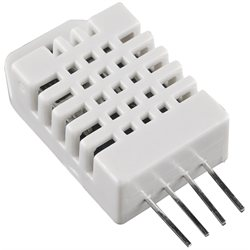
\includegraphics[scale=0.8]{./Figures/dht22.jpg}
        \rule{35em}{0.5pt}
    \caption[DHT22 sensor]{DHT22 humidity and temperature sensor.}
    \label{fig:DHT22}
\end{figure}


%------------------------------------
%	SUBSECTION 2 - MINI SOUND SENSOR
%------------------------------------

\subsection{Emartee Mini Sound Sensor}
\label{sub:sound}

Manufactured by Emartee, can also be found by the name of ``Emartee part number 4021'', and can be used to measure noise levels among other uses. Esentially, it consists on a microphone with a built-in amplifier onto a breakout board, which can be useful to work directly with perfboards or breadboards (both construction bases for rapid prototyping of electronic circuits).

The output signal is analog and is increased by a factor that allows an Arduino or any device with analog I/O pins to detect it easily\citep{gertz2012environmental}. Its operating voltage is 5V.


%------------------------------------
%	SUBSECTION 3 - SHARP DUST
%------------------------------------

\subsection{Sharp GP2Y1010AU0F}
\label{sub:sharp}

This is an inexpensive optical dust sensor, used to measure air quality. It is made out of an infrarred emitting diode which, with a well positioned phototransistor can measure the reflected IR rays thus detecting dust levels in the air\citep{sharp}. This device, which can be powered with up to 7V gives an output voltage (analog) proportional to dust density in the air. Some of its applications are air monitoring and air conditioning.

\begin{figure}[htbp]
    \centering
        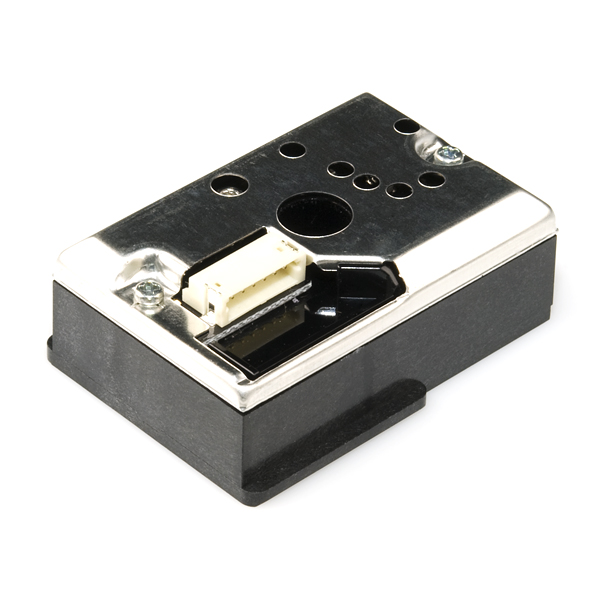
\includegraphics{./Figures/sharp.jpg}
        \rule{35em}{0.5pt}
    \caption[Sharp GP2Y1010AU0F]{Sharp GP2Y1010AU0F optical dust sensor.}
    \label{fig:SharpGP2Y1010AU0F}
\end{figure}

Surprisingly, this detector, which is priced at the time of writing about \$12, gives very precise results, similar to those offered by an expensive laser particle counter.\citep{airquality}


%-----------------------------------
%	SUBSECTION 4 - LM35
%-----------------------------------
\subsection{LM35}
% TODO


%----------------------------------------------------------------------------------------
%	SECTION 2 - XBEE MODULE
%----------------------------------------------------------------------------------------

\section{Digi XBee\textregistered{} Wireless RF Module}
\label{sec:xbee}

These radio modules are based on the IEEE 802.14.4 standard and provide an unexpensive, low power, low rate communication. They mainly use ISM\footnote{Descripción de ISM.} bands. 

\begin{figure}[htbp]
    \centering
    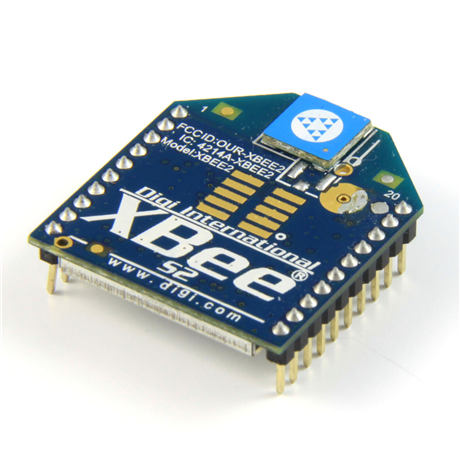
\includegraphics[scale=0.4]{./Figures/xbee.png}
        \rule{35em}{0.5pt}
        \caption[Digi XBee RF Module]{Digi XBee\textregistered{} Wireless RF Module}
    \label{fig:XBee RF Module}
\end{figure}

There are two versions of these modules, named ``Series 1'' and ``Series 2''. The older one (Series 1) implements the previously mentioned IEEE 802.15.4 standard which enables the network to follow point to point topologies. On the other hand however, the latter implements a standard specification called \emph{ZigBee}. This protocol, although more complex has mesh networking capabilities which can be a key feature in some sensor networks.

Despite their size provide us with many interesting features, such as 128-bit encryption, over-the-air configuration and several pins that enables the XBee to read analog values as well as working with digital input and output\citep{xbeedatasheet}.

This is why for the sake of this project ``Series 2'' has been chosen. It is worth saying that each of the two versions can transmit with different power levels thus varying the effective communication range\citep{faludi2010building}. More detailed information can be found in the table below.

% -T-A-B-L-E---- 
\begin{table}[ht] 
\centering
\begin{tabular}{l l l l}
    Version     & Power                 & Indoor range     & LoS range\footnotemark[1]\\
\hline
Series 1        & 1mW                   & 30m              & 100m\\
Series 1 PRO    & 63mW\footnotemark[2]  & 90m              & 1600m\\
Series 2        & 2mW                   & 40m              & 120m\\
Series 2 PRO    & 63mW\footnotemark[2]  & 90m              & 1500m\\
\end{tabular}
\caption{Comparison of different versions of XBee\textregistered.}
\end{table}

\footnotetext[1]{LoS range refers to line of sight range, where a straight line can be drawn from the transmitter to the receiver. In this situation, there are no obstacles between them and better bitrates and/or ranges can be achieved.}
\footnotetext[2]{This output power can be obtained using high gain antennas.}

Also, if extra range is needed (up to 40km in line of sight) there are also XBee\textregistered{} devices that transmit in lower ISM bands (900 and 868 MHz). However, when transmitting in these frequencies neither ZigBee nor IEEE 802.15.4 can be used. DigiMesh\texttrademark{} networking protocol is the only option and it is property of Digi International Inc.


%----------------------------------------------------------------------------------------
%	SECTION 3 - ARDUINO
%----------------------------------------------------------------------------------------

\section{Arduino}

Arduino is the leading protopying platform nowadays. It is completely open source including the schematics of the hardware itself, which is a single-board microcontroller. Anyone can program the board through a programming language very similar to C/C++ and based on \href{http://wiring.org.co}{Wiring}. To upload a sketch (a program) to the microcontroller they also have developed an Arduino IDE based on \href{htpp://processing.org}{Processing}.

The amount of projects related to this platform is incredibly big, and it has gained huge popularity amongst designers, hackers, programmers and hobbyists these past years. It offers several advantages over similar devices, because it is really cheap, cross-platform and has every benefit inherent to the open source initiative. Also, like other open projects Arduino comes in many ``flavours'' depending on the characteristics of the project.

As it can be seen on the next picture, the board has many input/output pins that are compatible with analog and digital values. It's not just that but also it can establish a serial communication with a computer so interaction between programs and the platform can take place.


\begin{figure}[htbp]
    \centering
    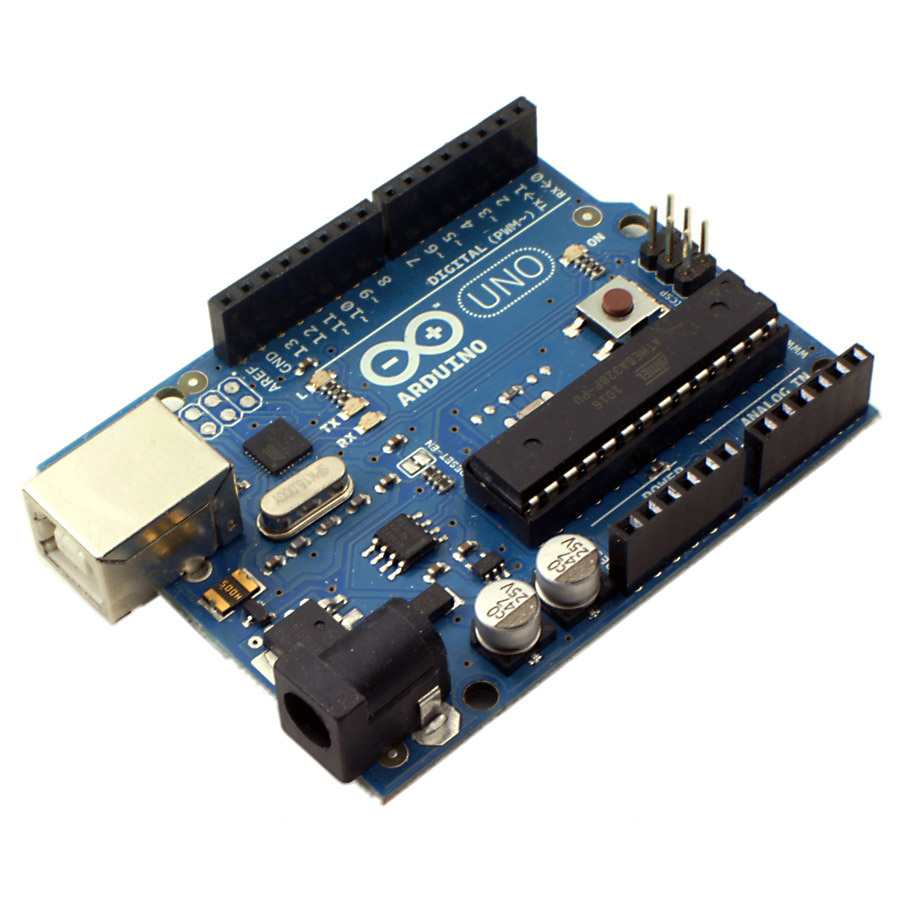
\includegraphics[scale=0.2]{./Figures/auno.jpg}
        \rule{35em}{0.5pt}
        \caption[Arduino UNO]{Arduino UNO prototyping platform.}
    \label{fig:ArduinoUNO}
\end{figure}

Arduino UNO is the one ``flavour'' that has been chosen to perform this project, since it is cheap and also the most common. That means all shields\footnote{A shield is another board plugged on top of the Arduino to extend its functionalities.}  work by default on it and the community it has is the biggest. In particular, this model has the following features\citep{arduinounor3}:
\\

\begin{table}[ht] 
\centering
\begin{tabular}{l|l}
    Feature     & Value\\
\hline
Microcontroller	& ATmega328\\
Operating Voltage &	5V\\
Input Voltage (recommended) & 7-12V\\
Input Voltage (limits) & 6-20V\\
Digital I/O Pins & 14 (of which 6 provide PWM output)\\
Analog Input Pins & 6\\
DC Current per I/O Pin & 40 mA\\
DC Current for 3.3V Pin & 50 mA\\
Flash Memory & 32 KB (ATmega328) of which 0.5 KB used by bootloader\\
SRAM & KB (ATmega328)\\
EEPROM &	1 KB (ATmega328)\\
Clock Speed &	16 MHz\\
\end{tabular}
\caption{Characteristics of the Arduino UNO.}
\end{table}


%----------------------------------------------------------------------------------------
%	SECTION 4 - RASPBERRY PI
%----------------------------------------------------------------------------------------
\section{Raspberry Pi}

This device is an inexpensive GNU/Linux box that follows an ARM architecture that acts as the sink of the network. There are two models of this device: one that has 256MB of RAM (known as model A), and another one that has 512MB of such memory (model B). As for the processor it utilizes a 700MHz Broadcom SOC. The operating system is directly loaded from an SD.

Currently it supports many popular distributions, such as: Arch GNU/Linux, Raspbian (a fork of Debian specifically designed to run on the Raspberry Pi), NetBSD, etc.

This is an optional part of the network since an XBee can be attached to any device that speaks serial. Nonetheless it is small and low-power, providing the necessary modularity for this kind of systems.

\begin{figure}[htbp]
    \centering
    \includegraphics[scale=0.2]{./Figures/pi.jpg}
        \rule{35em}{0.5pt}
        \caption[Raspberry Pi]{Raspberry Pi}
    \label{fig:RaspberryPi}
\end{figure}


%----------------------------------------------------------------------------------------
%	SECTION 5 - WI-FI DONGLE
%----------------------------------------------------------------------------------------
\section{D-Link DWA-123}

The Raspberry Pi, as stated before, has an ethernet interface, but in case such option cannot be used, a Wi-Fi dongle is the best solution. This model in particular is works out-of-the box with the Raspberry Pi and is cheap as well, supporting 802.11b/g/n.


%----------------------------------------------------------------------------------------
%	SECTION 6 - Arch GNU/Linux ARM
%----------------------------------------------------------------------------------------
\section{Arch GNU/Linux ARM}
Explicar.

%% Chapter Template

\chapter{Methodology} % Main chapter title

\label{Chapter4} % Change X to a consecutive number; for referencing this chapter elsewhere, use \ref{ChapterX}

\lhead{Chapter 4. \emph{Methodology}} % Change X to a consecutive number; this is for the header on each page - perhaps a shortened title

%----------------------------------------------------------------------------------------
%	JUST INTRO
%----------------------------------------------------------------------------------------

The first step I took to complete this project was having a deep look at the state of the art. There are a lot of sensor network designs and some are as well open sourced, but the majority of them require either advanced knowledge on PCB fabrication or are focused on just one particular area (they aim to solve just one problem). Thus developing a system which is multipurpose and uses well-known technologies for rapid deployment are some of the key requirements that this network should meet (apart from the initial objectives).

Once all initial requirements are identified I had to choose one appropriate life cycle for the project. The pilot scope was not strictly constrained thus changes shall be handled in some way. Consequently, I chose an agile\citep{} approach.

Agile management is a special case of iterative management, driven by changes\citep{pmbok_agile}. Development of small modules is the usual thing, with deadlines every two or four weeks. Also, stakeholders are highly involved which is very related to the approach we followed all the components of BuB4EU. Each month there was a scheduled workshop where every participant informed the rest of the team about his/her last advancements. This method is very useful for getting constant feedback hence improving the overall quality of the project.

At the same time, the pilot followed an open development model, since it was (and still is) available on GitHub from the beginning. Open projects present several advantages over closed ones\citep{}, such as: penisses.
 
%\chapter{Open Sensor Network}
\label{Chapter5}

\lhead{Chapter 5. \emph{Open Sensor Network}}

%----------------------------------------------------------------------------------------
%	INTRODUCTION
%----------------------------------------------------------------------------------------

The big picture objective of this project was to create a sensor network that allowed developers to gather real-time information from the Internet to create new solutions\citep{barcelobottom}. This chapter addresses how this main objective has been completed and dives into step-by-step explanations, from some ZigBee basic concepts (which are necessary to understand how the system works), to very detailed aspects related to the code, together with some flowcharts to visually interpret underlying features.

My contribution to the sensor network ecosystem is a set of tools to rapidly deploy such a system. More exactly:

\begin{itemize}
    \item XBee\textregistered{} configuration files. They are ready to be used and loaded into these RF modules.
    \item Fritzing\footnote{Fritzing is open source software that allows to design Arduino-based prototypes. The same software can be used to design final PCB boards from the initial prototyping view.} schematics, in order to replicate the nodes I worked with.
    \item Sink daemon code, used to receive all the information and then upload it to the Internet.
    \item Code of the Arduino program that will be running on some of the nodes.
    \item This document, which will guide everyone that wants to replicate or expand my work.
\end{itemize}

Technologies, as described in chapter \ref{Chapter3} are well-tested and mature solutions, thus inferring the project the following two main features:

% TODO . segundo punto
\begin{itemize}
    \item Flexibility --- The system is prepared to transmit heterogeneous information. Each node is able to transmit different information and the sink will decode it anyway. This allows a community to gather what each individual wants or to achieve better granularity where needed. That is, someone might be interested in measuring temperature every two blocks and humidity every four blocks.
    \item Velocity of deployment --- To deploy this network, just the RF modules must be properly configured, as well as some small code tweaking. In other words, just sensor nodes have to be adapted to particular needs, the sink will work anyway.
\end{itemize}


%----------------------------------------------------------------------------------------
%	SECTION 1
%----------------------------------------------------------------------------------------

\section{Network topology}

Network topology refers to the way nodes that conform the system are arranged, thus it is clear that this factor will determine very important components about the network, such as reliability, modularity, fault occurence, etc. The use of Digi Xbee\textregistered{} RF modules enables the network to be configured in any kind of topology, from a simple ring to a complex mesh\footnote{Networks where a packet can follow more than one path to reach its destination.}. An example of a mesh network is depicted in figure \ref{fig:MeshNet}, where each circle represents a node and the lines the wireless links between them.

\begin{figure}[htbp]
    \centering
        \includegraphics[scale=0.35]{./Figures/mesh_network.png}
        \rule{35em}{0.5pt}
    \caption[Mesh Network]{An example of a mesh network.}
    \label{fig:MeshNet}
\end{figure}

As these RF devices only allow one single sink per network, not making use of mesh topologies would be an enormous drawback, since packet delivery would be subject to other nodes availability. Luckily, ZigBee specification allows that some nodes act as a relay for other nodes, enabling us to build complex networks with redundant paths. This statement, translated to battery-powered systems means that the more relay nodes a network has, the more prolonged the network's lifetime will be\citep{hou2005energy}, since relay nodes will have to pass on less messages.


A mesh sensor network of this kind can be fully connected ---each node is connected to every other one--- or partially connected. This topology brings many advantages. They basically enable the system to be:

\begin{itemize}
    \item Self-healing --- Allows the network to operate when a node goes down.
    \item Self-routing --- When a packet is transmitted or forwarded, the route that it follows is created ---that is, calculated--- locally within every node.
    \item Self-forming --- Nodes that are new to the network create links automatically with the rest of nodes and routes are created dinamically as well.
\end{itemize}

The mentioned features and constraints imply that the first step to build such a network will begin by placing a sink and then start building from there, progressively reaching more distant places.

%-----------------------------------
%	SUBSECTION 1
%-----------------------------------
\subsection{Device roles}

Inside an ZigBee network there are three roles that a node can assume: coordinator, router and end device.

A \emph{coordinator} is the sink of the network, and as stated before, only one is allowed per network. A coordinator stores vital information about the network, acts as well as the trust center\footnote{Stores the keys if encryption is enabled, deciding who may or may not join the network.} and manages network security in general\citep{sensornetworktc}. In this case, it will be connected to the Raspberry Pi so data can be processed and uploaded to the Internet.

A \emph{router} can be understood as the previously mentioned relay nodes. It can generate and transmit data by itself to other router or to a coordinator but it is also able to forward packets from other nodes. If the network is very redundant it should not be a problem having a battery-powered router. If that is not the case, this option could lead to data outage, since packets from the edge of the network could not be forwarded.

Finally, an \emph{end device} is the least capable device of all. It can only transmit information that will be or will not be forwarded, thus they are always on the edge of the network. Since no other node depends on an end device, they can make use of the \emph{sleep mode}. This mode allows an XBee radio to wake up every certain amout of time, transmit whatever it has to and then go back to sleep again. This mode is very energy efficient.

An example of such a network can be seen in figure \ref{fig:ZBeeNet}.

\begin{figure}[htbp]
    \centering
        \includegraphics[scale=0.7]{./Figures/zigbee_topology.png}
        \rule{35em}{0.5pt}
        \caption[ZigBee network example]{An example of an ZigBee network, taken from the ZigBee Alliance website (\url{http://zigbee.org}).}
    \label{fig:ZBeeNet}
\end{figure}

%----------------------------------------------------------------------------------------
%	SECTION 2
%----------------------------------------------------------------------------------------

\section{Sensor nodes}

A sensor node is an element inside a wireless sensor network that is capable of gathering information, has some processing power and can relay information (if needed) to other nodes in the network\citep{chong2003sensor}.

In the design of this network two feasible scenarios have been considered, depending on which kind of sensors need to be used ---whether they are digital or analogic---, and if processing power is required. In case at least one of those features is needed, an Arduino plus an XBee\textregistered{} module are coupled together, with sensors attached to the board. Otherwise a standalone XBee\textregistered{} is used since it has a built-in ADC\footnote{An analog-to-digital converter takes a continous value --voltage, in our case-- as its input and converts it to a digital numeral.}, hence being able to directly read information from analog sensors.

These two operational modes have been taken in consideration because despite one of them can equate the other's characteristics one can think of some applications where the features of an additional microcontroller are just not needed. For instance, a sensor network monitoring temperature in an industrial environment just needs the so-mentioned analog-to-digital converter and a transceiver. Although there are two types of nodes, both can be used at the same time inside a given network.

To configure the radio of a sensor node one must use X-CTU, a piece of software developed by Digi International that, although it is intended to be run on Windows, it works fine on GNU/Linux using Wine\footnote{Wine is open source software that helps running Microsoft Windows applications on Unix-like operating systems.}, as it can be seen in figure \ref{fig:xctuonubuntu}.

In the next subsections it will be presented how these two types of sensor nodes are wired, how do they work, etc.

\begin{figure}[htbp]
    \centering
        \includegraphics[scale=0.6]{./Figures/xctuonubuntu.png}
        \rule{35em}{0.5pt}
        \caption[Screenshot of X-CTU]{A screenshot of X-CTU running on Ubuntu 12.04 under Wine.}
    \label{fig:xctuonubuntu}
\end{figure}

%-----------------------------------
%	SUBSECTION 1
%-----------------------------------
\subsection{Standalone XBee}

To collect data directly from an XBee\textregistered{}, we need to make use of the analog-to-digital converters mentioned in section \ref{sec:xbee}. In figure \ref{fig:XBeeBO} we can observe the pinout of an XBee radio, with all its DIO (digital input output) pins. For analog input, we can only use from \texttt{DIO0} (sometimes called as well \texttt{AD0}) to \texttt{DIO3} (or \texttt{AD3})\citep{faludi2010building}.

\begin{figure}[htbp]
    \centering
        \includegraphics[scale=0.25]{./Figures/xbee_breakout.jpg}
        \rule{35em}{0.5pt}
    \caption[XBee pinout]{XBee pinout, seen from a breakout board.}
    \label{fig:XBeeBO}
\end{figure}

An schematic of this node can be seen below (figure \ref{fig:StandaloneXBee}), where only light level and temperature are measured. This particular setup could be useful for example to prevent fires in forests (although the optimal setup should have a humidity sensor as well).

\begin{figure}[htbp]
    \centering
        \includegraphics[scale=0.6]{./Figures/standalonexbee.png}
        \rule{35em}{0.5pt}
    \caption[Standalone XBee]{A standalone XBee node.}
    \label{fig:StandaloneXBee}
\end{figure}

Here, with the help of four AAA batteries we power an XBee\textregistered{} as well as the other sensors placed in the prototyping board. The temperature sensor (subsection \ref{sub:lm35}) has a dedicated output pin, which is directly attached to an analog input pin. As for light levels, the used LDR resistance\footnote{A photoresistor whose resistance varies depending on the surrounding light level.} does not have an output pin, and this is why we have to collect the sensory value through a voltage divider.

Using a battery and a solar panel to power a sensor node like this one, along with \emph{sleep mode} can result in very long lifetimes.

% ###############################
% # CONFIGURING STANDALONE XBEE #
% ###############################
\subsubsection{Configuring a standalone XBee\textregistered{}}
\label{subsub:coxbee}

The first step is to flash the radio module with the correct firmware, that is, with the \texttt{XB24-ZB} firmware. This \texttt{ZB} firmware implements the ZigBee 2007 specification\footnote{At the time of writing, the latest specification is from 2012.}. Also, a function set (or role) has to be set, as shown in figure \ref{fig:xctuw}.

\begin{figure}[htbp]
    \centering
        \includegraphics[scale=0.6]{./Figures/xctuw.png}
        \rule{35em}{0.5pt}
        \caption[XBee\textregistered{} through X-CTU]{XBee\textregistered{} through X-CTU.}
    \label{fig:xctuw}
\end{figure}

To configure a standalone node one must ensure that the RF module has the same \texttt{PANID} than the coordinator ---that is, in the same network---. Also, API mode shall be enabled, thus setting the \texttt{AP} parameter to \texttt{2}, which means not only that API mode must be used but also \emph{escaping}.

With escaping mode enabled the system escapes some special characters. In other words, if special characters appear in the packet ---for instance \texttt{0x7E}, which serves as a start frame delimiter--- they are replaced by other sequences so they can be decoded as well by the receiver but without causing any trouble in the interpretation phase. Receiving an arbitrary \texttt{0x7E} could pose many problems for the receiver. It would not know when a packet really starts\citep{digi:escapedchars}.

Since we want to transmit samples periodically, we must configurate a sampling rate inside X-CTU, with the parameter \texttt{IR}. This value must be hexadecimal, so if for instance we want the module to transmit values every second, we must set \texttt{IR} to \texttt{3E8} ---or 1000ms---.

Finally, parameters \texttt{D0}, \texttt{D1}, \texttt{D2} and \texttt{D3} can be set to \texttt{2}, which will mean they are in ADC mode. In other words, for each sensor wired to one of these pins, one must configure those pins to work in the proper mode.

% TODO - Adjust repo
Example configuration files were exported from X-CTU and can be freely downloaded from the original git repository\footnote{\url{https://github.com/aandreuisabal/OSN}}. More precisely, they can be found in the \texttt{Config/X-CTU} folder.

%-----------------------------------
%	SUBSECTION 2
%-----------------------------------
\subsection{Arduino-based node}

Arduino is capable of executing C code, thus being able to process any kind of information no matter how complex it is (always bearing in mind its hardware limits). To transmit all the information, the RF module attached to it will be configured as described in subsection \ref{sub:xbeearduino}.

As a proof of concept, the example setup I have worked with has an analog sensor that measures sound levels (\ref{sub:sound}), another one that measures air quality in terms of fine particles in the air (\ref{sub:sharp}) and a digital sensor that reads humidity and temperature (\ref{sub:dht}). A possible setup with these elements is shown in figure \ref{fig:ArduinoNode}.

Here, the Arduino board can be powered by batteries or by a more stable power supply. It is the very same board that powers the sensors and the XBee\textregistered{}. Thereby, information is gathered and finally transmitted through the RF module (more information in section \ref{subsub:arduinosketch}).

% TODO - Conseguir modelo de Fritzing para SHARP GP2Y1010AU0F
\begin{figure}[htbp]
    \centering
        \includegraphics[scale=0.8]{./Figures/completesensornode.png}
        \rule{35em}{0.5pt}
    \caption[Arduino-based node schematic]{Sensor node based on Arduino.}
    \label{fig:ArduinoNode}
\end{figure}

This type of node has the same communication features as the standalone XBee. That is, encryption, acknowledgements, etc. Additionally, ACKs are better handled in this case since an Arduino can \emph{react} to them.

%-----------------------------------
%	SUBSUBSECTION 1
%-----------------------------------
\subsubsection{XBee\textregistered{} configuration}
\label{sub:xbeearduino}

The configuration for this type of node is quite simple. The same firmware and function set that were mentioned in subsection \ref{subsub:coxbee} have to be written in the XBee\textregistered{}.\texttt{PANID} must be set to the same than the coordinator's so they can interact with each other, and \texttt{AP} (that is, API mode) must be set to \texttt{2} to enable escaping.

%-----------------------------------
%	SUBSUBSECTION 2
%-----------------------------------
\subsubsection{Arduino sketch}
\label{subsub:arduinosketch}
A sketch is nothing more than the program an Arduino runs. The basic code is written in C/C++, and it consists of a main file ---with \texttt{.ino} extension--- and the XBee\textregistered{} libraries. The code can be browsed and downloaded via GitHub. There are two versions of the sketch:

\begin{itemize}
    \item Exact same code I used to conduct the experiments, so anyone can verify and/or test the obtained results.
    \item A skeleton file, that follows a very minimalistic approach in terms of lines of code but fully commented. This way, it can be extended as desired to build a sensor network from scratch with customized sensor nodes.
\end{itemize}

Arduino IDE is based on Processing IDE\footnote{\url{http://processing.org}}, and it follows the same structure than the Processing programming language. There are two main functions necessary for every program to work, namely \texttt{setup()} and another one called \texttt{loop()}. Respectively:

\begin{itemize}
    \item The \texttt{setup()} funcion initializes variables, modules (such as the XBee), libraries and sets pins in specific modes. After this function is successfully executed \texttt{loop()} is immediately called.
    \item \texttt{loop()} is a function that as its own name indicates, is executed over and over again. Thus inside this structure is where the action takes place. 
\end{itemize}

In our case, before even \texttt{setup()} starts, the following steps take place:

\begin{itemize}
    \item An object of type \texttt{XBee} is created, so serial information can be exchanged between the microcontroller and the RF module. 
    \item Additional information useful for the transmission is set: destination address (by default \texttt{0x0000000000000000}\footnote{This address is used to simply reach the coordinator. It is possible to write the specific address of the XBee ---which is written in the RF module--- as well.}), how big the packet will be, etc.
    \item Also, an array called \texttt{payload} is initialized, which will contain all readings as well as some \emph{metadata}. 
    \item The variables that will hold the different readings are also declared outside the two main function so they are recognized in a global scope.
    \item Finally, auxiliary C unions\footnote{An union allows us to represent information in more than one way. In our case it helps us convert integers, booleans, etc. into byte-level data.} are created. One for every compatible data type.
\end{itemize}

In our \texttt{setup()} step we initialize a serial connection with the XBee\textregistered{} and set a pin to act as digital output. This pin is the number \texttt{13}, which is connected to the on-board LED.

Then, in \texttt{loop()} all sensory values are recollected and then transmitted via a ZigBee packet. Finally, if the previously mentioned LED blinks once that will mean transmission took place successfully, otherwise it will blink twice. This last feature is especially interesting when debugging.

In figure \ref{fig:ArduinoProgram} it is depicted how the program works in more detail. This flowchart follows a top-down approach. That is, from general to more specific functions.

\begin{figure}[htbp]
    \centering
        \includegraphics[scale=0.43]{./Figures/SensorNodeDia.png}
        \rule{35em}{0.5pt}
    \caption[Flow diagram of an Arduino-based node]{Flow diagram of the Arduino program.}
    \label{fig:ArduinoProgram}
\end{figure}

As for how values are read from the Arduino, figure \ref{fig:readvalues} explains how this process takes place step by step. Basically, digital values are read one time since the readings are more precise, and when reading an analog value the Arduino computes an average of \texttt{n} samples to smoothe the values from ``jumpy'' sensors.

\begin{figure}[htbp]
    \centering
        \includegraphics[scale=0.38]{./Figures/readvalues.png}
        \rule{35em}{0.5pt}
    \caption[Value reading flowchart]{Flowchart of how values are read.}
    \label{fig:readvalues}
\end{figure}

\paragraph{Working with metadata}
~\\
An initial requirement was that each sensor node can transmit whatever it needs to, I designed a rudimentary but efficient mechanism. At the start of every packet, an integer is sent. This is the only fixed value that every packet will hold. This integer will be tremendously helpful so the sink knows how to decode the payload ---keep in mind that data is sent in binary form---.

That is, the four first bytes of payload of every packet will be decoded as an unsigned integer at the sink --- which ranges from $0$ to ($2^{16}-1$)---. Then, each digit that conforms this number will be interpreted (one by one) as a unique data type, using table \ref{tab:mapnumbers}. The range of this unsigned integer is bigger when using other flavors of the Arduino, such as the Arduino Due\footnote{\url{http://arduino.cc/en/Guide/ArduinoDue}}.

\begin{table}[ht] 
\centering
\begin{tabular}{c|l}
Number          & Data type             \\
\hline
1               & \texttt{boolean}      \\
2               & \texttt{char}         \\
3               & \texttt{unsigned char}\\
4               & \texttt{int}          \\
5               & \texttt{unsined int}  \\
6               & \texttt{long}         \\
7               & \texttt{unsigned long}\\
8               & \texttt{short}        \\
9               & \texttt{float}        \\
0               & \texttt{double}       \\
\end{tabular}
\caption{Mapping between numbers and data types.}
\label{tab:mapnumbers}
\end{table}

To come up with an actual way to translate between digits and data types, I had a look at which data types the Arduino IDE could handle, and which of them Python can decode ---that is, which data types do they share---. For more information on supported data types one can visit the reference on the official Arduino webpage\footnote{\url{http://arduino.cc/en/Reference/HomePage}} and Python documentation on data structures\footnote{\url{http://docs.python.org/2/library/struct.html}}.

To give an example, let's say a node wants to transmit two floats and a boolean. According to table \ref{tab:mapnumbers}, this would yield the numbers \texttt{9}, \texttt{9} and \texttt{1}. Hence this number (\texttt{METADATA} in the code) can be \texttt{199}, \texttt{919} and so on. 

Nonetheless, it is recommended to first transmit the lowest values (starting with \texttt{1},\texttt{2}\ldots) and finishing with the highest ones (\ldots\texttt{9},\texttt{0}). This is because since the range of an \texttt{unsigned int} is somewhat small ---at least in a 8-bit architecture--- transmitting information in this order reduces the probabilities or exceeding that range (which would lead to errors).

In the current state of the code, this ``magic'' number has to be hardcoded. Once this number has been written in the \texttt{METADATA} variable, the information shall be sent in the same order. Following the previous example, this number would be \texttt{199}, thereby sending the boolean first and then the two remaining floats.

\paragraph{Packing information}
~\\
Information is packed with the help of unions, as stated before. A union is declared as follows:

\begin{verbatim}
union u_boolean {
    uint8_t b[1];
    boolean boolean;
} boolean_union;
\end{verbatim}

This means that the union named \texttt{boolean\_union} will translate indifferently between a boolean and a byte. Later on, the \texttt{payload} variable ---which as its own name indicates, holds the payload--- shall be filled with the data (including the metadata):

\begin{verbatim}
boolean_union.boolean = sample_boolean;
for (int i=0;i<BOOLEAN_SIZE;i++){
    payload[i]=boolean_union.b[i];
}
\end{verbatim}

Although these lines of code seem ``messy'' at first clange its functionality is quite simple. It just loads the payload with byte information.


%----------------------------------------------------------------------------------------
%	SECTION 3
%----------------------------------------------------------------------------------------

\section{Network sink}

The sink is where all the information is headed. As stated in the previous section, it is composed of a Raspberry Pi with an XBee module connected to it. The schematic, although simple can be seen in the figure \ref{fig:sinkrpi}. Note that in the figure there is not an XBee but a breakout board for it that has a miniUSB interface, very useful for our purposes. On top of it there is the actual XBee\textregistered{}.

\begin{figure}[htbp]
    \centering
        \includegraphics[scale=0.7]{./Figures/server_side.png}
        \rule{35em}{0.5pt}
    \caption[Raspberry Pi based sink]{Schematic of the sink.}
    \label{fig:sinkrpi}
\end{figure}

The GNU/Linux distribution that has been chosen to operate in this device is Arch Linux ARM, as stated in section \ref{sec:alarmmm}. Its repositories are huge because regular users contribute to a non-official repository, called ``Arch User Repository'' (also known as AUR). There, all the packages mentioned in chapter \ref{Chapter3} are available without compiling from source ---in the form of binaries---.

The script, called \texttt{server.py} is then run as a daemon which will be always receiving information. It needs two arguments:

\begin{itemize}
    \item Device file that interfaces with the XBee\textregistered{} (e.g. \texttt{/dev/ttyUSB0}). Depending on the devices already attached to the computer the last number might change.
    \item Baud rate the XBee\textregistered{} is working at (e.g. \texttt{9600}). Can be customized via X-CTU.
\end{itemize}

What the script basically does is run an asynchronous \texttt{XBee} dispatcher, which will create a new background thread for every new packet that arrives, thus enabling the sink to process many packets at the same time without blocking the whole script. The program is quite modular, since it allows to upload the information to the website the user wants by just uncommenting certain lines. A more detailed view on how it generally works can be seen in figure \ref{fig:sindia}.

\begin{figure}[htbp]
    \centering
        \includegraphics[scale=0.44]{./Figures/sindia.png}
        \rule{35em}{0.5pt}
    \caption[Flow diagram of the sink script]{Flow diagram of the sink script.}
    \label{fig:sindia}
\end{figure}

However, in figure \ref{fig:sindia} we cannot appreciate how packets are actually handled, and what happens to them afterwards. For that matter, figures \ref{fig:phandler} and \ref{fig:puploader} explain these two phases more precisely.

\begin{figure}[htbp]
    \centering
        \includegraphics[scale=0.38]{./Figures/packet_handler.png}
        \rule{35em}{0.5pt}
    \caption[Packet dispatcher flowchart]{Flowchart of how packets are dispatched.}
    \label{fig:phandler}
\end{figure}

\begin{figure}[htbp]
    \centering
        \includegraphics[scale=0.38]{./Figures/packet_uploader.png}
        \rule{35em}{0.5pt}
    \caption[Packet uploader flowchart]{How a packet uploader works.}
    \label{fig:puploader}
\end{figure}

At the moment of writing, two uploaders have been created. One for Xively\footnote{\url{http://xively.com}} and one for any Nimbits cloud\footnote{\url{http://nimbits.com}}. The results can be seen in chapter \ref{Chapter6}.

\subsection{Setting up the sink}

The XBee\textregistered{} settings that have to be set are the same that those on an Arduino node. That is, a certain \texttt{PANID} and the \texttt{AP} parameter set to \texttt{2}.

These are the steps related to the Raspberry Pi that have to be followed to get a functioning sink:

\begin{enumerate}
    \item Get a compatible SD card\footnote{\url{http://elinux.org/RPi_SD_cards}}, download the latest ISO image from the Arch Linux ARM website\footnote{\url{http://archlinuxarm.org/platforms/armv6/raspberry-pi}} and transfer it to the card. Depending on what operative system you are using you will want to use one tool or another. If the operating system is correctly loaded in the SD card the Raspberry Pi shall boot properly and its LEDs will start blinking.
    \item To actually interact with the device, there are two options:
        \begin{itemize}
            \item Through a display that accepts HDMI input and a USB keyboard.
            \item Arch Linux ARM has the SSH\footnote{Secure Shell allows to remotely access another machine and remotely execute commands.} daemon enabled by default.
        \end{itemize}
    \item Arch Linux makes use of \texttt{pacman}, a wonderful package manager. From a terminal, issue the following command (requires root access): 
        \begin{verbatim}
            pacman -Syu python2 python2-requests python2-pyserial
        \end{verbatim}
    This will upgrade all the operating system packages and will install as well the necessary ones for the script to work.
    \item Clone the GitHub repository by issuing: 
        \begin{verbatim}
            git clone https://github.com/aandreuisabal/OSN.git
        \end{verbatim} 
    This will clone the GitHub repository. More precisely, inside the \texttt{Code/server} folder there are all the necessary files to run the sink daemon.
\end{enumerate}



%----------------------------------------------------------------------------------------
%	SECTION 4
%----------------------------------------------------------------------------------------
\section{Deploying the network}

To deploy this network one must first configure the coordinator as explained before, and start placing sensor nodes ---configured properly--- around until reaching the desired coverage. As for the script, one must first fill the necessary constants, such as API keys ---necessary to upload information to data clouds---, usernames, etc.
 
%\input{./Chapters/Chapter6} 
%\input{./Chapters/Chapter7} 

%----------------------------------------------------------------------------------------
%	THESIS CONTENT - APPENDICES
%----------------------------------------------------------------------------------------

\addtocontents{toc}{\vspace{2em}} % Add a gap in the Contents, for aesthetics

\appendix % Cue to tell LaTeX that the following 'chapters' are Appendices

% Include the appendices of the thesis as separate files from the Appendices folder
% Uncomment the lines as you write the Appendices

% Appendix A

\chapter{Appendix Title Here} % Main appendix title

\label{AppendixA} % For referencing this appendix elsewhere, use \ref{AppendixA}

\lhead{Appendix A. \emph{Appendix Title Here}} % This is for the header on each page - perhaps a shortened title

Write your Appendix content here.
%\input{./Appendices/AppendixB}
%\input{./Appendices/AppendixC}

\addtocontents{toc}{\vspace{2em}} % Add a gap in the Contents, for aesthetics

\backmatter

%----------------------------------------------------------------------------------------
%	BIBLIOGRAPHY
%----------------------------------------------------------------------------------------

\label{Bibliography}

\lhead{\emph{Bibliography}} % Change the page header to say "Bibliography"

\bibliographystyle{unsrtnat} % Use the "unsrtnat" BibTeX style for formatting the Bibliography

\bibliography{Bibliography} % The references (bibliography) information are stored in the file named "Bibliography.bib"

\end{document}  
